\section{Level Design}
In this section the sequences of the implemented level "Giant Chasm" are explained. The level is divided into 5 sequences.\\
Under the representative map of the section are listed all the dialogues belonging to that specific time section.

\subsection{Level Map (First Sketch)}

\begin{figure}[H]
	\centering
	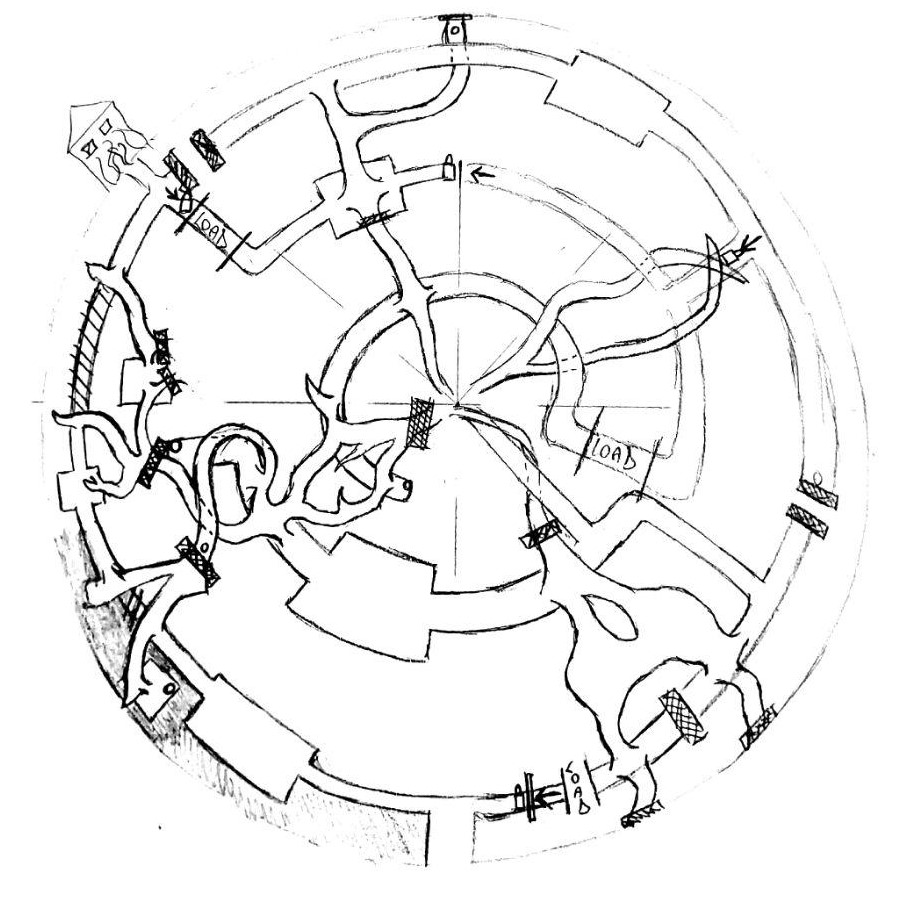
\includegraphics[width=0.8\linewidth]{images/visual_ref/15_giant_chasm/chasm_map.jpg}
	\caption*{Complete map of the level (Boss Room excluded)}
\end{figure}

\begin{figure}[H]
	\centering
	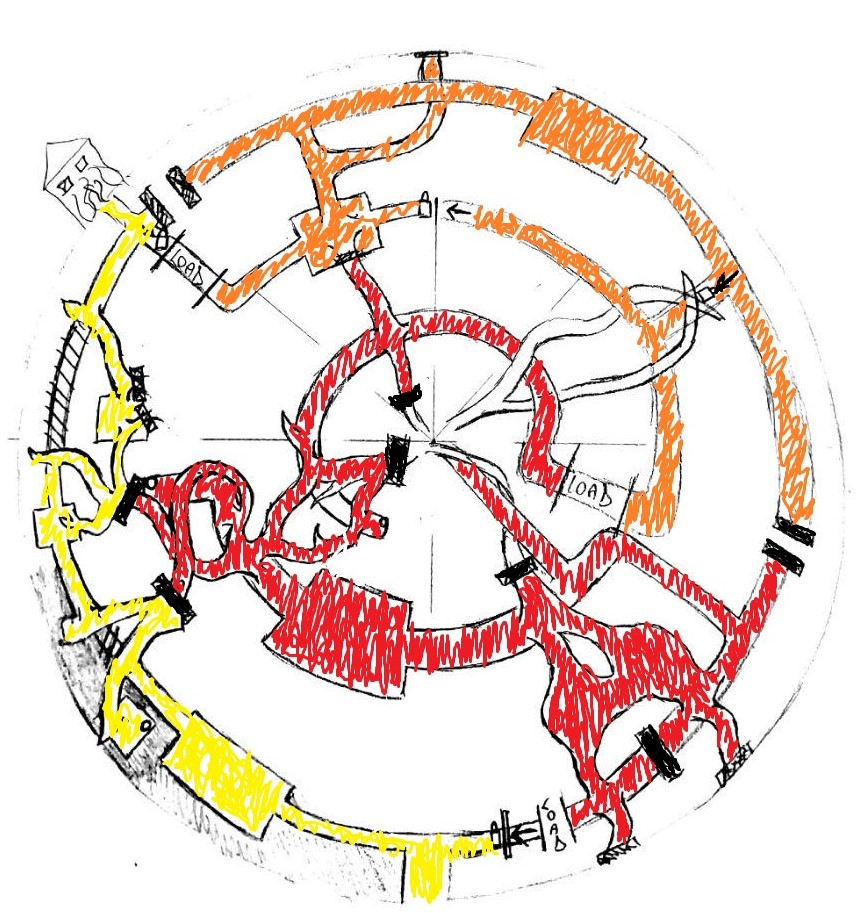
\includegraphics[width=0.8\linewidth]{images/visual_ref/15_giant_chasm/chasm_colored_map.jpg}
	\caption*{Section 1: Yellow, Section 2: Orange, Section 3: Red}
\end{figure}

\subsection{Visual References}

\subsubsection{Giant Chasm Outside}

\begin{figure}[H]
	\centering
	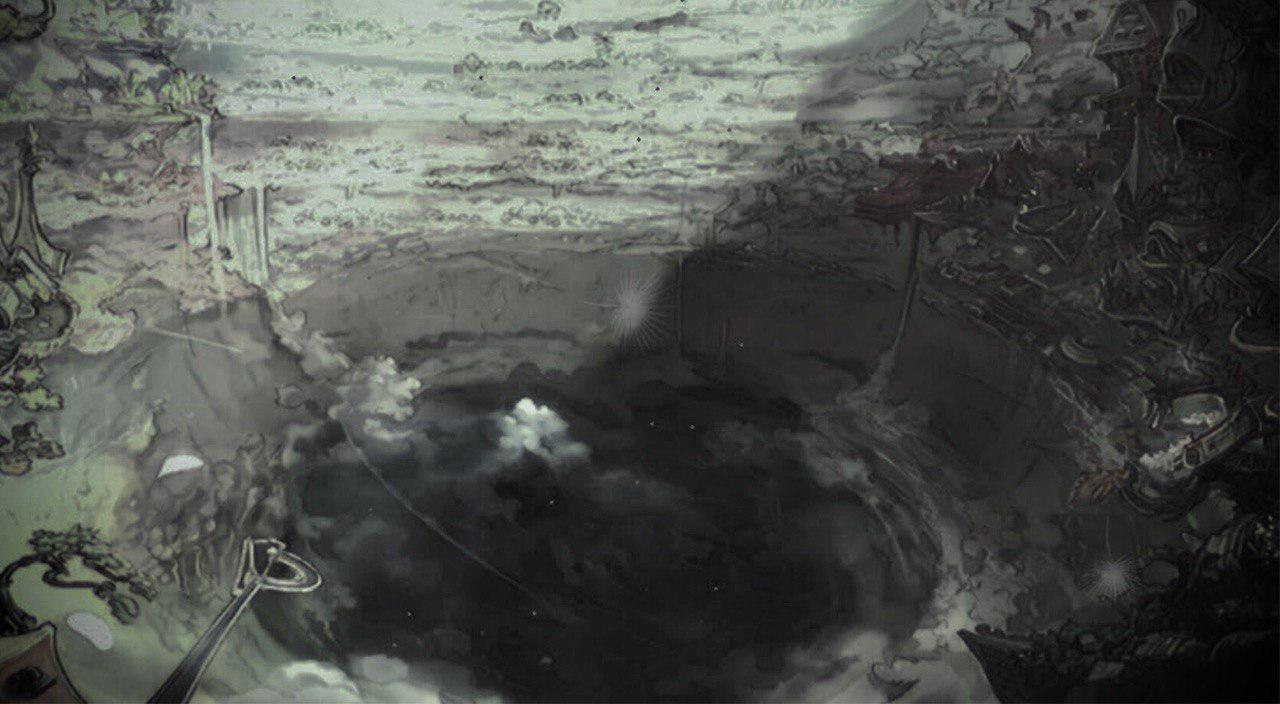
\includegraphics[width=0.8\linewidth]{images/visual_ref/15_giant_chasm/chasm_outside.jpg}
	\caption*{Overview of the Giant Chasm. \textit{[Made in the Abyss]}}
\end{figure}

\subsubsection{Giant Chasm Section 1 \& 2}

\vspace*{0.3cm}
\begin{figure}[H]
	\centering
	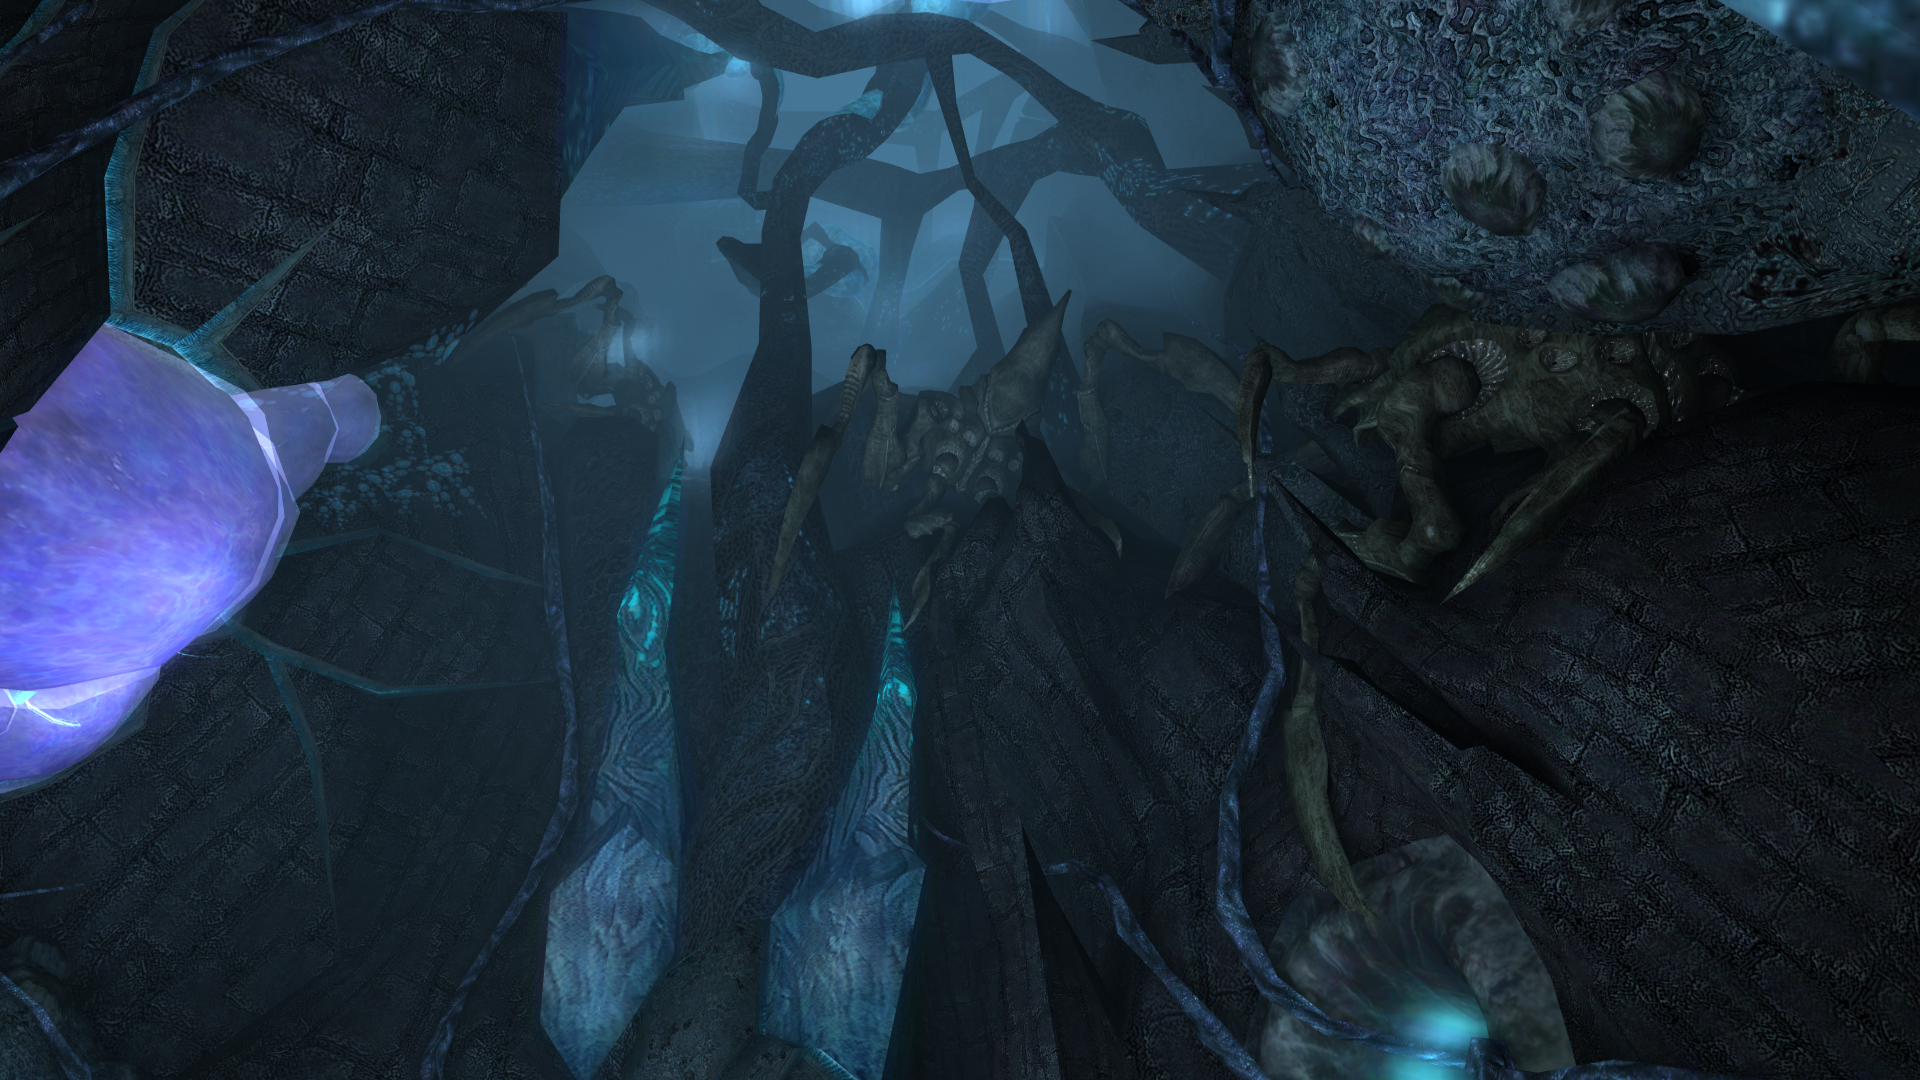
\includegraphics[width=0.8\linewidth]{images/visual_ref/15_giant_chasm/chasm_section_1_2.png}
	\caption*{Path of the first and second section}
\end{figure}

\subsubsection{Giant Chasm Section 3}

\vspace*{0.3cm}
\begin{figure}[H]
	\centering
	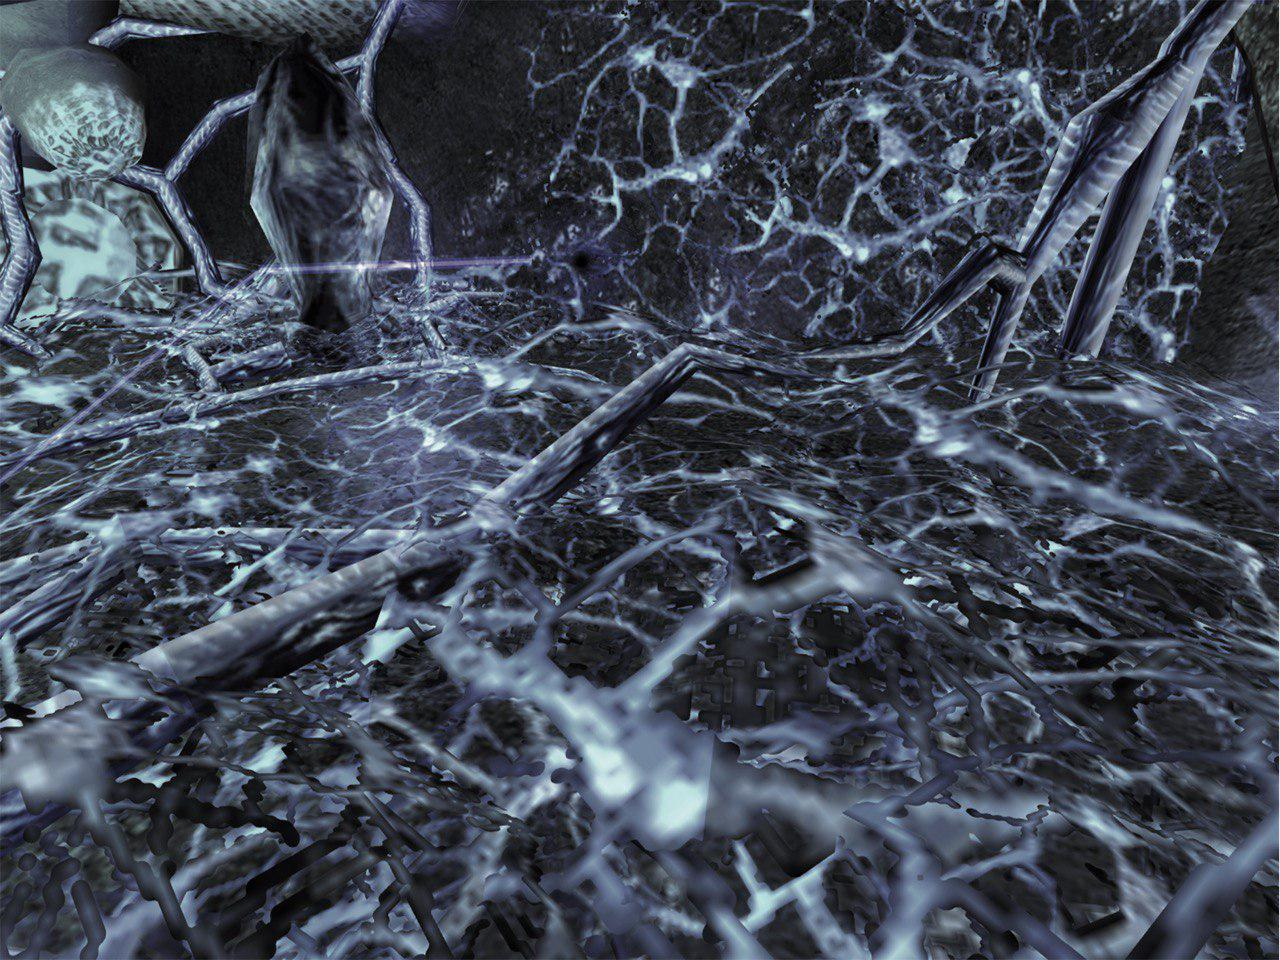
\includegraphics[width=0.8\linewidth]{images/visual_ref/15_giant_chasm/chasm_section_3.jpg}
	\caption*{Ground in the third section}
\end{figure}

\subsubsection{Giant Chasm Core}

\vspace*{0.3cm}
\begin{figure}[H]
	\centering
	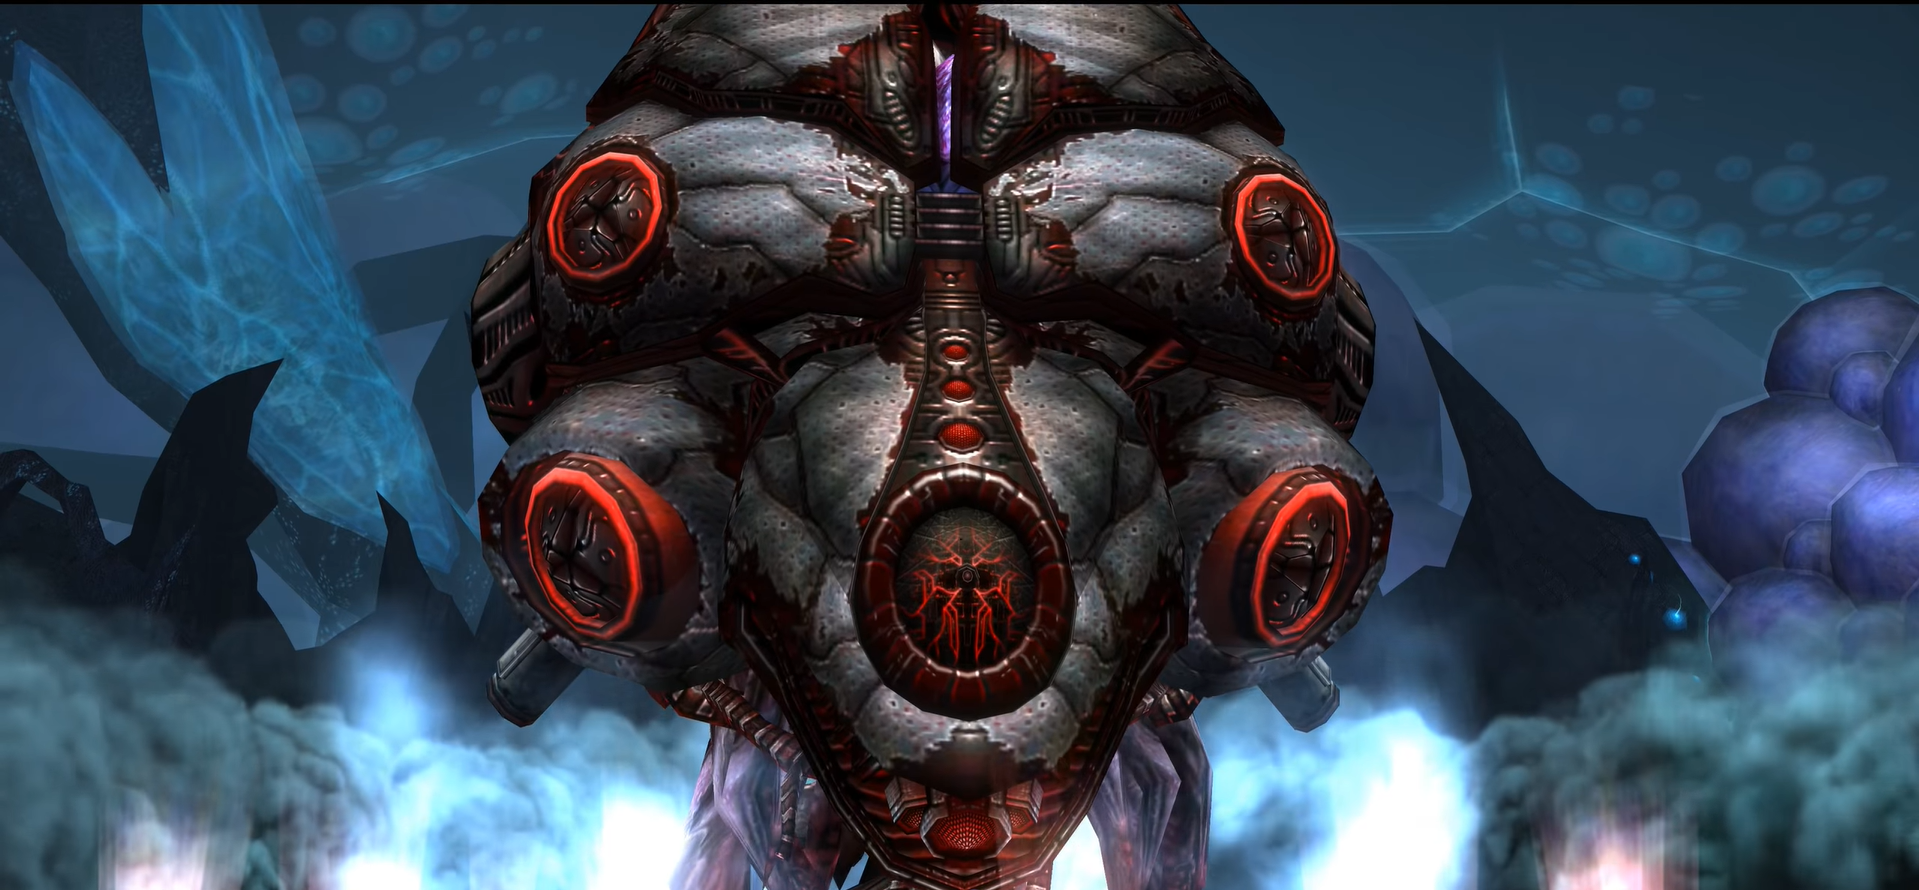
\includegraphics[width=0.8\linewidth]{images/visual_ref/15_giant_chasm/chasm_core.png}
	\caption*{Core of the Upside-Down (in-game it will be more organic and it will emit more red light)}
	\caption{ \textit{[Metroid Prime]}}
\end{figure}

\subsection{Dialogues}

\subsubsection{Section 1}
\vspace*{0.3cm}

	\textbf{Entered the Giant Chasm, Elby and \#010 remain stunned by the dense network of ramifications that cover the whole area.}

\begin{dialogue}
	
	\speak{\#010} \direct{Astonished} \textit{"So this is the place where the core of the upside-down resides. It looks like a giant crater, it is possible that ..."}
	\speak{Elby} \textit{"I have no time or interest in your hypotheses, we must reach Kyle."}
	\speak{\#010} \textit{"Oh, you're right ... I see a light in the center, I think it's our destination"}\\
	
	\textbf{After a quick inspection, the two decide to continue along the edge and look for a route to the center.}\\
	
	If the player tries to go on the right:
	\speak{\#010} \textit{"This tangle of branches is too thick, we will not be able to pass this way. Let's find another path."}\\
	
	\textbf{Reached the remains of a building that collapsed inside the crater, Elby and 10 arrive in what appears to be
an old ballroom. Suddenly they hear the roars of monsters, which appear one after another around them.}\\
	
	
	\speak{\#010} \direct{Worried} \textit{"We are in their den after all, just try to save as much stamina as possible!"}\\
	
	\textbf{Once the monsters are defeated, they continue along the cliff to reach a second room divided in half
from a pit.}\\
	
	\speak{\#010} \textit{"I don't think I can jump so much, I'm sorry ..."}
	\speak{Elby} \textit{(That branch ... Maybe with my skills I can create a path)}\\
	
	\textbf{After using his telekinesis to cross the pit, Elby and \#010 follow the ramifications to continue on the track until they reach a third room, where they find several monsters impaled by branches.}\\
	
	
	\speak{\#010} \textit{"All these pierced monsters, I think it was \refer{\#001.}"}
	\speak{Elby} \textit{"You should be happy."}
	\speak{\#010} \textit{"Why?"}
	\speak{Elby} \textit{"..."}
	\speak{\#010} \textit{"Ah, if he killed them it means he doesn't have the power to control them, so \refer{\#005} is still alive!"}
	\speak{Elby} \direct{Nods towards \refer{\#010}}\\
	
	
	\textbf{Once at a dead end, they begin to look for a route inland.}\\
	
	
	\speak{\#010} \textit{"This is the only point from which we could descend, but the branches are too thick! Do you have any ideas?"}
	\speak{Elby} \direct{Looks around}
	\speak{Elby} \direct{Indicates a building on the edge of the crater}
	\speak{Elby} \direct{Smiling}\textit{"Freeze it"}
	\speak{\#010} \direct{Excited} \textit{"Maybe by combining our skills we can bring it down. Let's try!"}\\
	
	
	\textbf{After freezing the branches that stabilized the structure and having destroyed them by means of telekinesis, the building begins to collapse and the debris, after rolling along the wall, hit the barrier of branches, opening a gap.}\\
	
	
	\speak{\#010} \textit{"Now we can pass, but let's stay on guard."}
	
\end{dialogue}


\subsubsection{Section 2}
\vspace*{0.3cm}

\begin{dialogue}
	\speak{\#010} \direct{Coff coff}
	\speak{Elby} \textit{"The density of the air has changed, we are getting closer"}\\
	
	Entering the Safe Room:
	\speak{\#010} \direct{Relieved}\textit{"We should be safe in here, we can make a brief stop to regain strength"}\\
	
	Leaving the Safe Room:
	\speak{\#010} \textit{"Let's go, we should be halfway there"}
\end{dialogue}


\subsubsection{Section 3}
\vspace*{0.3cm}


	\textbf{The proximity to the core is increasingly evident: the ground is completely covered with organic branches and the air density is skyrocketing.}

\begin{dialogue}
	
	
	\speak{\#010} \textit{"We're getting closer to the core, the light that emanates is much more intense than before"}
	\speak{Elby} \direct{Angered} \textit{"Don't distract yourself!"}
	\speak{\#010} \textit{"Sorry!"}\\
	
	
	\textbf{Unable to follow the ground path, Elby and \#010 decide to continue the journey using the ramifications of the core as a route}\\
	
	\speak{\#010} \textit{"The branching of the core is extremely dense at this point"}
	\speak{Elby} \textit{"We are almost there"}\\
	
	Section one link, post skill:
	\speak{\#010} \textit{"We can now reach the entrance from here"}
	\speak{Elby} \direct{nods}\\
	
	
	\textbf{Finally they arrive on a non-natural path, certainly created by Kyle to reach the center of the giant chasm.}\\
	
	\speak{\#010} \textit{"\refer{\#001} must be close, are you ready?"}
	\speak{Elby} \textit{"Yes"} or \textit{"Not yet"}\\
	
	If answer is "Yes":
	\speak{\#010} \textit{"Ok, let's go ..."}\\
	
	If answer is "Not yet":
	\speak{\#010} \textit{"Make it quick, \refer{\#005} needs us!"}
	
\end{dialogue}


\subsubsection{Inner Section}
\vspace*{0.3cm}

\begin{dialogue}
	
	\speak{\#010} \textit{"\#001!"}
	\speak{Kyle} \direct{Joking} \textit{"Oh, finally. I was starting to think you were dead along the way!"}
	\speak{\#005} \direct{Squirms}
	\speak{Kyle} \textit{"Hey hey, calm down, wait for your turn"}\\
	
	If the player has visited Kyle's lab:
	\speak{\#010} \textit{"We've been in your lab, we know what you've done and what you are up to!"}
	\speak{Kyle} \textit{"So you found out everything ... Great, you saved me a lot of explanations"}\\
	
	If the player has not visited Kyle's lab:
	\speak{\#010} \textit{"Why all this?"}
	\speak{Kyle} \textit{"I just want back what was taken from me, nothing more"}\\
	
	\speak{\#010} \textit{"And are you going to kill us all for your purpose?"}
	\speak{Kyle} \textit{"Not everyone, just the two of them in case they don't want to cooperate" \direct{Points \refer{Elby} and \refer{\#005}}}
	\speak{Kyle} \textit{"By the way, you are staring at me with a fierce look, do you have something to say?" \direct{Watching \refer{Elby}}}
	\speak{Elby} \direct{Really angered} \textit{"Friends ... don't ... LIE !!!"} \direct{Gust of energy}
	\speak{Kyle} \textit{"Haha, so you consider me a friend, how nice!"}
	\speak{Kyle} \direct{Serious look}
	\speak{Kyle} \textit{"Chatting time's over, now give me your powers!"}
	
\end{dialogue}

\subsubsection{After Boss Fight}
\vspace*{0.3cm}

\begin{dialogue}
	\speak{Kyle} \textit{"... The effect of the core is more intense than I thought ..."}
	\speak{Elby} \textit{"Free \#005. NOW!"}
	\speak{Kyle} \textit{"..."}
	
	\textbf{The costrinctions around 005 are released, allowing him to move.}\\
	
	\speak{\#005}: \textit{"Thank y-"}\\
	
	\textbf{\#005 stops moving and suddenly blood starts to come out of his mouth.}\\
	
	\speak{Kyle} \textit{"You didn't give me a choice."}\\
	
	\textbf{A branch pierces the chest of \#005, extracting a DemoParasite.}\\
	
	\speak{\#010} \direct{Desperate look and vomit from horror}
	\speak{Elby} \direct{Tear from left eye}
	\speak{Kyle} \textit{"And now ..."}
	\speak{Kyle} \direct{swallows the DemoParasite}
	\speak{Kyle} \direct{closes his eyes}\\
	
	\textbf{Elby launches a mental attack, but a barrier of branches block it}\\
	\speak{Elby} "???!!?"
	\speak{Kyle} \direct{Open his eyes}
	\speak{Kyle} \textit{"I have control over the core, there's nothing more you can do."}\\
	
	\textbf{The whole Giant Chasm begins to tremble. In a few moments, hundreds of branches emerge from the ground, trapping Elby and \#010.}\\
	
	\speak{Kyle} \textit{"If you do not want to follow the same fate as \refer{\#005} do not resist and open the portal"}\\
	
	\textbf{A branch wraps around the neck of \#010, starting to strangle him}\\
	
	\speak{Elby} \direct{Initially reluctant} \textit{"Okay. I'll do it ..."}
	\speak{Kyle} \textit{"Great!"}\\
	
	\textbf{Kyle closes his eyes again, entering a state of deep concentration. Suddenly, the air inside the core changes, almost as if all the space there was in a continuos changing state}\\
	
	\speak{Kyle} \textit{"The time is right. Go on!"}\\
	
	\textbf{Elby starts to focus. The chasm begins to tremble again and in few seconds a portal appears in the room. Kyle watches it with a satisfied look and tears running down his face.}\\
	
	\speak{Kyle} \textit{"Now i can finally go home ..."}
\end{dialogue}